\chapter{Security and Privacy}
\begin{figure}[htbp]
   \centering
   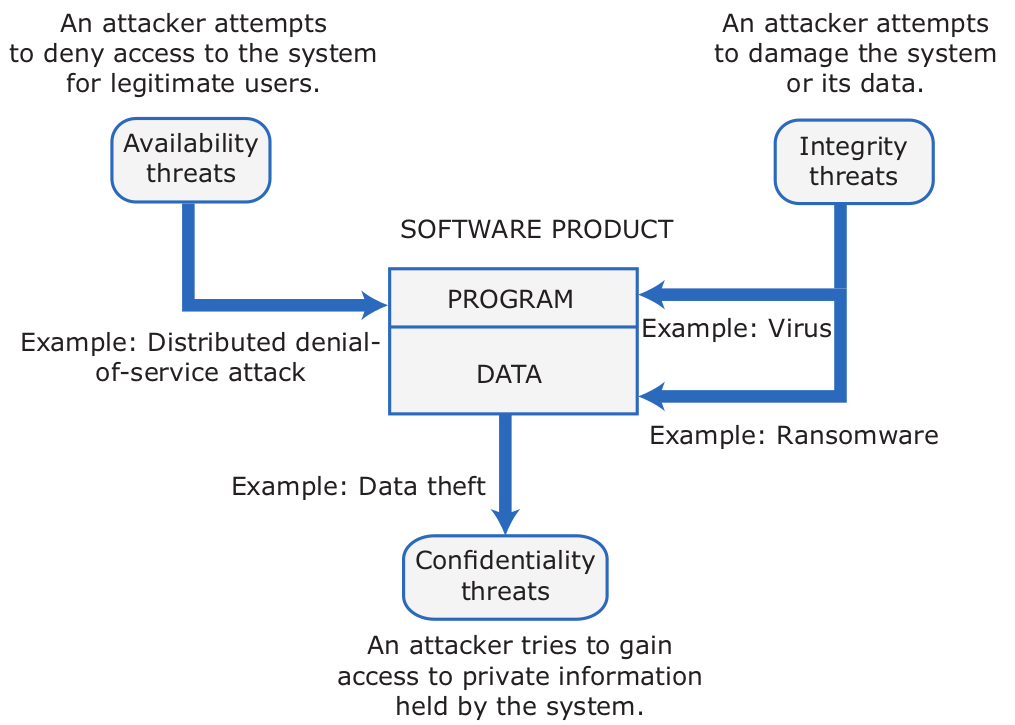
\includegraphics{images/security_threats.png}
   \caption{Security threats}
   \label{fig:security_threats}
\end{figure}
\textbf{Security} is a \textit{system-wide issue}:
Application software depends on operating system, web server, language run-time system, database, frameworks and tools, which may \textit{all} be targeted by attacks.

There are some system management procedures whose aim is to increase security, 
the most obvious ones are \textbf{authentication} and \textbf{authorization} (later discussed in Sections \ref{sec:authentication} and \ref{sec:authentication}).
\textit{System infrastructure management} aims to keep infrastructure software configured
and to promptly apply security updates patching vulnerabilities.
Regularly \textit{monitoring attacks} enhances the ability to detect them and trigger resistance strategies to minimize the impact.
To achieve resilience instead, \textit{backup policies} are defined to keep undamaged copies of program and data files to be restored after an attack.
\section{Attacks types}

\subsection{Injection Attacks}
Malicious users try to crash the system by sending invalid input values.
The defense is definining a robust input validation.

\labelitemize{
   \textit{Examples}
}{
   \begin{enumerate}
      \item Buffer overflow attacks
      \item SQL Poisoning
   \end{enumerate}
}

\subsection{Session hijacking}
A \textit{Session} is a time period during which user's auth with a web app is valid;
it allows the user to not having to re-authenticate for subsequent system interactions.
A session is closed when the user logs out or due to a “times out” caused by
no user inputs for some time. 

An attacker may acquires a valid session cookie through \textit{Cross-site scripting} (\textit{active} hijacking) or \textit{traffic monitoring} (\textit{passive} hijacking), and then impersonate a legitimate user.

Possible defenses include:
\begin{itemize}
   \item Encryption (\texttt{HTTPS})
   \item Multifactor authentication
   \item Short timeout sessions
\end{itemize}

\subsubsection{Cross-site Scripting}
\texttt{XSS} (i.e. \textit{cross-site scripting}) falls in the category of injection attacks,
since it consists in adding malicious code {---}to leak information{---} to a web page returned from a server to a user,
which inputs precious data handled by the malware.

\subsection{Denial-of-Service attacks}
\textbf{DoS} are intended to make system unavailable for normal use,
and were typically implemented by sending a high number of requests to overload servers,
resulting in the unavailability of services provided by such servers.

An historical \textbf{DoS} technique exploited the TCP 3-way handshake.
DoS developed in \textit{Distributed DoS} (\textbf{DDoS}),
i.e. sending requests from multiple IP addresses.

The most basic DoS techniques now have standard countermeasures to block them.
Widely used basic countermeasures include:
\begin{enumerate}
   \item IP tracking
   \item Temporary users lockout after failed authentication
\end{enumerate}

\subsection{Brute Force}
Attackers may try to guess missing authentication information by generating all possible combinations of characters,
possibly by knowing partial information on the string to be generated.


\section{Authentication}
\label{sec:authentication}
\labelitemize{
   \textit{Approaches}
}{
   \begin{enumerate}
      \item \textbf{Knowledge}-based authentication\\
      Personal secret knwon by the user.\\
      Passwords are often insecure, forgotten, reused,
       and besides the user can be fooled into inserting it in fake websites (\textit{phishing}).
      \item \textbf{Possession}-based authentication\\
      Possessing a physical device which provides tokens.
      \item \textbf{Attribute}-based authentication\\
      Biometric information of the user.
      \item \textbf{Multi-factor}:\\
      Combining the above. 
      This is becoming way more common and standardized.
   \end{enumerate}
}

\section{Authorization}
\label{sec:authorization}
\textbf{Authorization} involves checking that an authenticated user can \textit{access resources},
while \textbf{authentication} is only about ensuring that the user is who they claim to be.

\textit{Access Control Lists} (\texttt{ACL}s) are widely used to implement access control policies,
they allow
classifying individuals into groups, dramatically reducing ACLs size,
and definining hierarchies of groups.\\
ACLs often realized by relying on ACL of underlying file or db
system.

\section{Encryption}

Encryption means making a document unreadable by applying an algorithmic transformation to it.
Modern encryption techniques are considered “practically uncrackable”
using currently available technology.

There are well-known symmetric and asymmetric encryption techniques.
\texttt{HTTPS} uses server-client interaction to generate a secret for symmetric encryption.\\
$\texttt{HTTPS} = \texttt{HTTP} + \st{\texttt{SSL}}\ \texttt{TLS}$ \textit{(Transport Layer Security)}\\
TLS is used to verify \textit{identity} of web server and to encrypt communications,
it does so by exploiting a digital certificate sent from server to client, issued by a trusted identity verification service (\texttt{CA}).

In general encryption should be adopted \textbf{whenever possible},
for both \textit{in transit} and \textit{at rest} data,
while for \textit{in use} data it is known that may cripple performance, 
and mechanisms of key management are used instead.

Ideally, if keys get lost, encrypted data become permanently inaccessible.
Keys should be changed periodically and multiple timestamped versions of keys should be mantained,
creating the need for a \textbf{Key Management System}
(\textit{KMS}) to make sure that keys are securely generated, stored, and accessed by authorized users.

\begin{figure}[htbp]
   \centering
   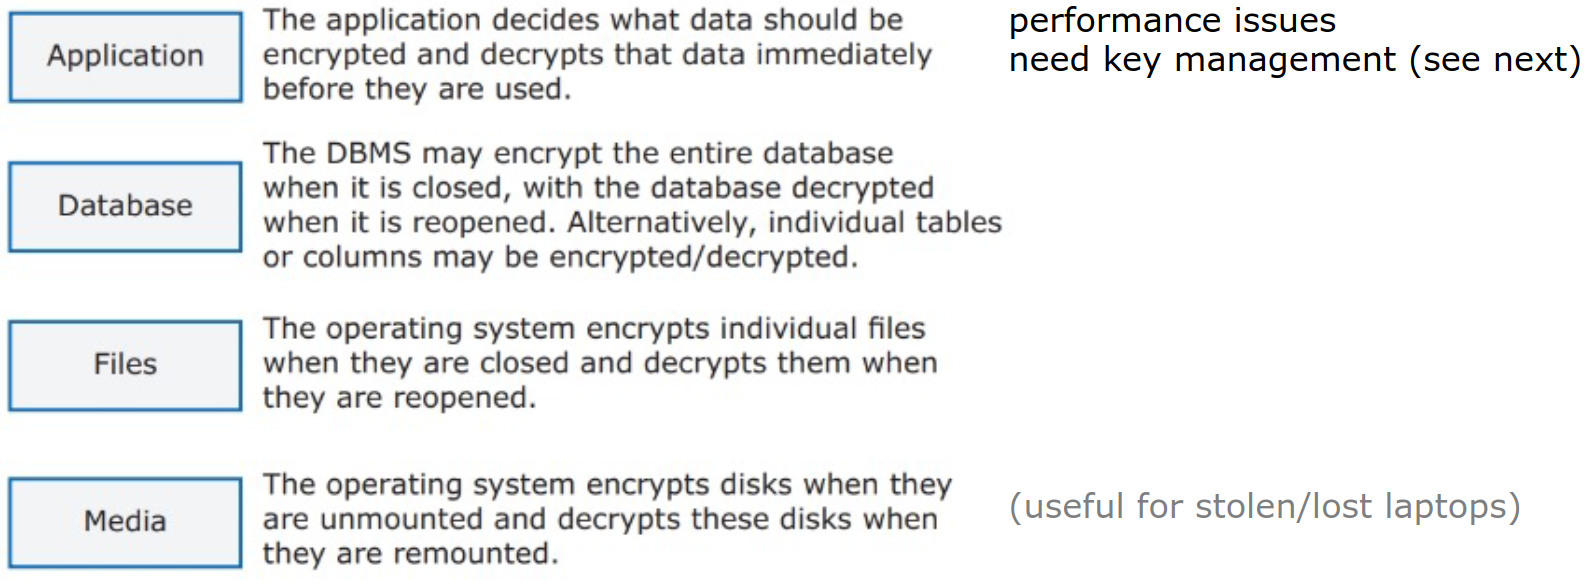
\includegraphics{images/encryption.png}
   \caption{Encryption is possible in all system levels}
   \label{fig:encryption}
\end{figure}

\section{Privacy}
\textbf{Privacy} is a social concept that relates to the collection,
dissemination, and appropriate use of personal information held
by a third party.

There may business reasons for paying attention to information privacy:
\begin{itemize}
   \item If your conformance to privacy regulations does not match data
   protection regulations, you may be subject to legal actions / cannot sell
   your product
   \item If your sell a business product, your business customers may require privacy safeguards (not to be at risk with their users)
   \item Leakage/misuse of client information can damage your reputation
\end{itemize}

The information that your software \textit{needs} to collect depends on the
\textit{functionality} of your product and on the business model you use;
we can provide some tips based on this assumption:
\begin{itemize}
   \item Do not collect personal information that you do not need
   \item Establish a privacy policy defining how personal/sensitive information about
   users is collected, stored, and managed
   \item Make clear if you use users’ data to target advertising or to provide services that are paid for by other companies
   \item If your product includes social network functionalities so that users can share
   information, you should ensure that users understand how to control the
   information they share
\end{itemize}